\documentclass[12pt,a4paper]{article}
\usepackage[utf8]{inputenc}
\usepackage[T1]{fontenc}
\usepackage{amsmath}
\usepackage{amsfonts}
%\usepackage{amssymb}
\usepackage{bbm}
\usepackage{graphicx}
\usepackage{geometry}
\usepackage{enumitem}
\usepackage{hyperref}

\usepackage{exsheets}
\SetupExSheets{counter-format=ch.qu}

\geometry{a4paper, margin=2cm}

\usepackage{cprotect}

\usepackage{xcolor}
\definecolor{maroon}{cmyk}{0, 0.87, 0.68, 0.32}
\definecolor{halfgray}{gray}{0.55}
\definecolor{ipython-frame}{RGB}{207, 207, 207}
\definecolor{ipython-bg}{RGB}{247, 247, 247}
\definecolor{ipython-red}{RGB}{186, 33, 33}
\definecolor{ipython-green}{RGB}{0, 128, 0}
\definecolor{ipython-cyan}{RGB}{64, 128, 128}
\definecolor{ipython-purple}{RGB}{170, 34, 255}

\usepackage{listings}
\lstdefinelanguage{iPython}{
	morekeywords={access,and,del,except,exec,in,is,lambda,not,or,raise},
	morekeywords=[2]{for,print,abs,all,any,basestring,bin,bool,bytearray,callable,chr,classmethod,cmp,compile,complex,delattr,dict,dir,divmod,enumerate,eval,execfile,file,filter,float,format,frozenset,getattr,globals,hasattr,hash,help,hex,id,input,int,isinstance,issubclass,iter,len,list,locals,long,map,max,memoryview,min,next,object,oct,open,ord,pow,property,range,reduce,reload,repr,reversed,round,set,setattr,slice,sorted,staticmethod,str,sum,super,tuple,type,unichr,unicode,vars,xrange,zip,apply,buffer,coerce,intern,elif,else,if,continue,break,while,class,def,return,try,except,import,finally,try,except,from,global,pass, True, False},
	sensitive=true,
	morecomment=[l]\#,%
	morestring=[b]',%
	morestring=[b]",%
	moredelim=**[is][\color{black}]{@@}{@@},
	identifierstyle=\color{black}\footnotesize\ttfamily,
	commentstyle=\color{ipython-cyan}\footnotesize\itshape\ttfamily,
	stringstyle=\color{ipython-red}\footnotesize\ttfamily,
	keepspaces=true,
	showspaces=false,
	showstringspaces=false,
	rulecolor=\color{ipython-frame},
	frame=single,
	frameround={t}{t}{t}{t},
	backgroundcolor=\color{ipython-bg},
	basicstyle=\footnotesize\ttfamily,
	keywordstyle=[2]\color{ipython-green}\bfseries\footnotesize\ttfamily, 
	keywordstyle=\color{ipython-purple}\bfseries\footnotesize\ttfamily
}

\lstdefinelanguage{iOutput} {
	sensitive=true,
	identifierstyle=\color{black}\small\ttfamily,
	stringstyle=\color{ipython-red}\small\ttfamily,
	keepspaces=true,
	showspaces=false,
	showstringspaces=false,
	rulecolor=\color{ipython-frame},
	basicstyle=\small\ttfamily,
}

\lstnewenvironment{ipython}[1][]{\lstset{language=iPython,mathescape=true,escapeinside={*@}{@*}}%
}{%
}

\lstnewenvironment{ioutput}[1][]{\lstset{language=iOutput,mathescape=true,escapeinside={*@}{@*}}%
}{%
}

\title{Addons with Python Exercises}
\author{Matteo Sani}

\begin{document}
\maketitle

\section{Simulating Stochastic Differential Equations}

Consider a generic stochastic differential equation (SDE)

\begin{equation}
dX(t) = \mu(t,X(t))dt + \sigma(t,X(t))dW(t)
\label{eq:sde}
\end{equation}

The Monte Carlo simulation of such a process can be carried out according to the \emph{Euler scheme} as follows: conisider the value of $X$ at time $t=t_i$, the value compute $X(t_{i+1})$ is evaluated from the dynamics of X (Eq.\ref{eq:sde}), setting $\Delta t = t_{i+1} - t_{i}$, and sampling from a standard normal $\mathcal{N}(0,1)$ in order to "evolve" the stochastic term $dW$
\begin{equation}
X(t_{i+1}) = X(t_i) + \mu(t_i,X(t_i))\Delta t + \sigma(t_i,X(t_i))\sqrt{\Delta t}\mathcal{N}(0,1)
\end{equation}

In the specific case of a simple brownian motion the dynamics is given by
\begin{equation}
dW = \sqrt{dt}\mathcal{N}(0,1)
\end{equation}
so
\begin{equation}
W(t+dt) = W(t) + \sqrt{dt}\mathcal{N}(0,1)
\end{equation}
or
\begin{equation}
W(t) = \sum_{t_0}^{t} \sqrt{dt}\mathcal{N}(0,1)
\end{equation}

Figure|\ref{fig:brownian_motion} reports two realization of the Brownian motion simulated according to the Euler scheme.

\begin{figure}[htbp]
\begin{center}
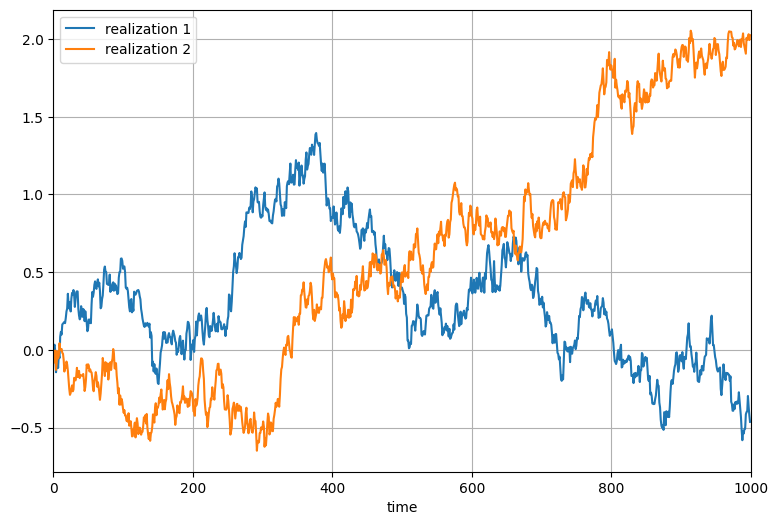
\includegraphics[width=0.5\linewidth]{addons/brownian_motion}
\end{center}
\label{fig:brownian_motion}
\end{figure}

\begin{question}
Using the Euler scheme simulate the 4-months (with daily steps) evolution of a Geometric Brownian Motion stochastic process with initial value $S_0=100$, $\mu=0.005$, and $\sigma=0.05$.
\end{question}

\cprotEnv\begin{question}
This \href{https://github.com/matteosan1/advanced_financial_modeling/raw/master/input_files}{file} contains a thousand 10-day realizations (with 0.1 day step) of historical price data of a single asset, assume that all the time series are different realizations of the same stochastic process.
\begin{itemize}
\item Make two figures: the first should contain one realization as a function of time, in the second plot the first 50 realizations together as a function of time (\emph{label the axes appropriately}).
\item In two separated plots report the mean and the variance of the stock prices as a function of time (\emph{label the axes appropriately}).
\item Perform the variable change $X_{n+1}=\log\left(\cfrac{S_{n+1}}{S_n}\right)$ on $S_{n+1} = S_ne^{(\mu-0.5\sigma^2)\Delta t + \sigma\sqrt{\Delta t}Z}$ to rewrite the model into a simpler form. 
	\begin{itemize}
	\item Is the resulting dynamics linear ? Prove it, or give a counterexample; 
	\item is the resulting system time-invariant ? Prove it, or give a counterexample.
	\end{itemize}
\item Apply again the same transformation $X_{n+1}=\log\left(\frac{S_{n+1}}{S_n}\right)$ to data this time. Plot both the mean and the variance of the transformed realizations as a function of time.
\end{itemize}

\noindent
\textbf{Hint:} the input file is a binary file that can be loaded back using \texttt{numpy} as follows (replace the URL from the link above):
\begin{ipython}
import numpy as np

path = np.DataSource("https://github.com/matteosan1/...../input_files")
S = np.load(path.open("stock_2023.npy", "rb"))
\end{ipython}
\end{question}

\section{Floating Rate Notes}
Floating rate bond or note (FRN) usually refers to an instrument whose coupon is based on a short term rate (3-month T-bill, 6-month LIBOR). Variable coupon rates are fixed in advance at reset dates, which are 3- or 6-month (interest payment period) earlier.

In this example we use an annual payment frequency but the extension to the quarterly or semi-annual frequency is straightforward.

Floating rate bond price with (\emph{unit notional amount}), $n$ maturity, annual frequency ($\tau=1$), and the first coupon rate predetermined at previous reset date ($C_{reset}$) is as follows.

\begin{equation}
\begin{aligned}
\textbf{FRN} & = D_{0,1}C_{reset} + \sum_{i=1}^nD_{0,i}f_{i,i+1} + D_{0,n}= \\
& = D_{0,1}C_{reset} + D_{0,2}f_{1,2} + \ldots + D_{0,n-1}f_{n-2,n-1}+ D_{0,n}(1+f_{n-1,n}) = \\
& = D_{0,1}C_{reset} + D_{0,2}\left(\frac{D_{0,1}}{D_{0,2}}-1\right) + \ldots \\
&\quad\ldots + D_{0,n-1}\left(\frac{D_{0,n-2}}{D_{0,n-1}}-1\right) + D_{0,n}\left(\frac{D_{0,n-1}}{D_{0,n}}-1\right) + D_{0,n} = \\
& = D_{0,1}C_{reset} + (D_{0,1} - D_{0,2}) + (D_{0,2} - D_{0,3}) + \ldots \\
&\quad\ldots + (D_{0,n-2} - D_{0,n-1}) + (D_{0,n-1} - D_{0,n}) + D_{0,n} = \boxed{D_{0,1} (1 +C_{reset})}
\end{aligned}
\end{equation}
where $f(t_1,t_2)$ denotes the forward rate between $t_1$ and $t_2$.

If the remaining maturity of the above \textbf{FRN} for example was 4.25 year, its price will be
\begin{equation}
\textbf{FRN} = D_{0,\frac{1}{4}}(1+C_{reset})
\end{equation}

If the remaining maturity of the above \textbf{FRN} was $(4 + \epsilon)$ year, in this case, the price would be

\begin{equation}
\begin{aligned}
\textbf{FRN} &= D_{0,1}f_{0,1}+ D_{0,2}f_{1,2} + \ldots + D_{0,n-1}f_{n-2,n-1} + D_{0,n}(1+f_{n-1,n}) = \\
& = D_{0,1}\left(\frac{D_{0,0}}{D_{0,1}}-1\right) + D_{0,2}\left(\frac{D_{0,1}}{D_{0,2}}-1\right) + \ldots \\
&\quad\ldots + D_{0,n-1}\left(\frac{D_{0,n-2}}{D_{0,n-1}}-1\right) + D_{0,n}\left(\frac{D_{0,n-1}}{D_{0,n}}-1\right) + D_{0,n} = \\
&= (D_{0,0}-D_{0,1})+(D_{0,1}-D_{0,2}) + \ldots \\
&\quad\ldots + (D_{0,n-2}-D_{0,n-1})+(D_{0,n-1}-D_{0,n})+D_{0,n} = 1
\end{aligned}
\end{equation}

The price of FRN has a range from \emph{par} to \emph{par} + full coupon. It is par right before the reset date and is $C$ right after the reset date (and is linear when pricing date is between two reset dates).

\begin{question}
Draw a plot showing the characteristic sawtooth behaviour of a floating rate note. The relevant insterest rates can be taken from \href{https://raw.githubusercontent.com/matteosan1/advanced\_financial\_modeling/master/input_files/libor.csv}{libor.csv}
\end{question}

\section{Importance Sampling}
Assume we want to calculate the expectation $\mathbb{E}[f(X)]$
\begin{equation}
\mathbb{E}[f(X)] = \int_{-\infty}^\infty f(x)p(x)dx
\end{equation}
where $p(x)$ is the probability density function associated to the random variable $X$.

We can approximate this expectation using numerical approximation, i.e. Monte Carlo simulation, by sampling $n$ random values from the distribution $p$ and then calculating the sample mean as:
\begin{equation}
\bar{f}(x) = \frac{1}{n}\sum_i f(x_i)
\end{equation}

The idea behind \textbf{importance sampling} is to use a simple re-formulation trick and write the expectation in a slightly different form
\begin{equation}
\mathbb{E}[f(X)] = \int_{-\infty}^\infty f(x)\frac{p(x)}{q(x)}q(x)dx
\end{equation}
giving the expectation of $f(x)\frac{p(x)}{q(x)}$ over the distribution $q$. And with that, allowing us to calculate the sample mean by sampling from $q$:
\begin{equation}
\bar{f}(x) = \frac{1}{n}\sum_i f(x_i)\frac{p(x)}{q(x)}
\label{eq:reformulated_expectation}
\end{equation}

\subsection{Variance Reduction}
From probability theory we know that the variance of the standard Monte Carlo estimator is given by:
\begin{equation}
\cfrac{1}{n}\cdot\text{Var}[f(x)] = \cfrac{1}{n}\cdot\mathbb{E}[(f(X)-\mathbb{E}[f(X)])^2]
\end{equation}

Hence the variance for the re-formulated importance sampling estimator in Eq.\ref{eq:reformulated_expectation} is:
\begin{equation}
\cfrac{1}{n}\cdot\text{Var}\left[\cfrac{p(x)}{q(x)}f(x)\right]
\end{equation}

This give us a hint on how to find a way to reduce the variance. And indeed it is relatively easy to see that this variance could be reduced to 0 by choosing $q$ as:
\begin{equation}
\begin{aligned}
q(x)&=\cfrac{f(X)p(x)}{\mathbb{E}[f(X)]} \implies \cfrac{1}{n}\cdot\text{Var}[\mathbb{E}[f(X)]] = \cfrac{1}{n}\cdot\mathbb{E}[(\mathbb{E}[f(X)]-\mathbb{E}[\mathbb{E}[f(X)]])^2]=\\
&=\cfrac{1}{n}\cdot\mathbb{E}[(\mathbb{E}[f(X)]-\mathbb{E}[f(X)])^2] = 0
\end{aligned}
\end{equation}

Naturally, we don’t know $\mathbb{E}[f(X)]$, as the reason we are doing this sampling after all is to find the expectation of $f$.
However, we can think of the denominator of the previous expression as some normalisation constant, and consider to construct $q$ such that it has \textbf{high} density wherever $f(x)p(x)$ is \textbf{high}.

\subsection{Practical Example}
For the sake of demonstration, we choose $f=\mathcal{N}(5, 1)$, and the probability distribution $p=\mathcal{N}(9,2)$ which do not overlap too well, see Fig.\ref{fig:f_and_p}.
\begin{figure}[htbp]
\begin{center}
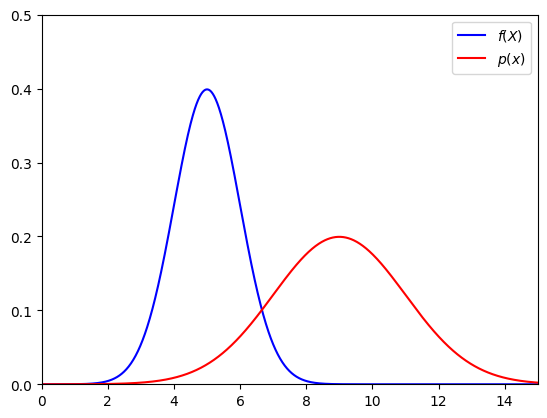
\includegraphics[width=0.5\linewidth]{addons/f_and_p}
\end{center}
\label{fig:f_and_p}
\end{figure}

To approximate numerically the expectation, as stated above, we would now sample values $x_i$ from the distribution $p$, and compute the mean of $f(x_i)$.

Intuitively one can see why sampling from this distribution is a bad idea: for most values sampled from $p$, $f$ will be close to 0, but for a few sampled values $f$ will be very large, thus we obtain a large variance.

\begin{figure}[htbp]
\begin{center}
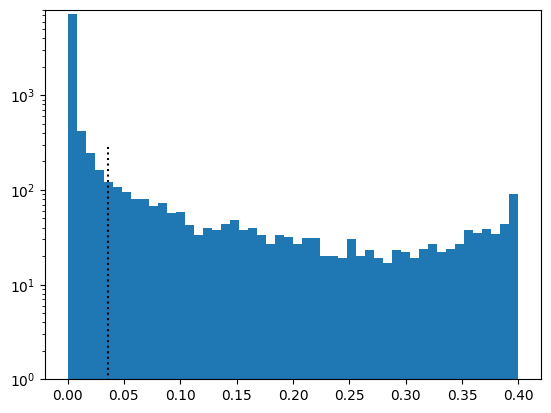
\includegraphics[width=0.5\linewidth]{addons/bad_sampling}
\end{center}
\label{fig:bad_sampling}
\end{figure}

Looking at Fig.|\ref{fig:bad_sampling} it is apparent how the vast majority of samples piles up at 0 (notice the logarithmic scale of the plot). 
Therefore, as outlined above, to make the sampling more efficient, we can try a new distribution $q = \mathcal{N}(5.8, 1)$, which satisfies the criterion that its pdf is high in regions where $f(x)p(x)$ is high, see Fig|\ref{fig:fp_and_q}.

\begin{figure}[htbp]
\begin{center}
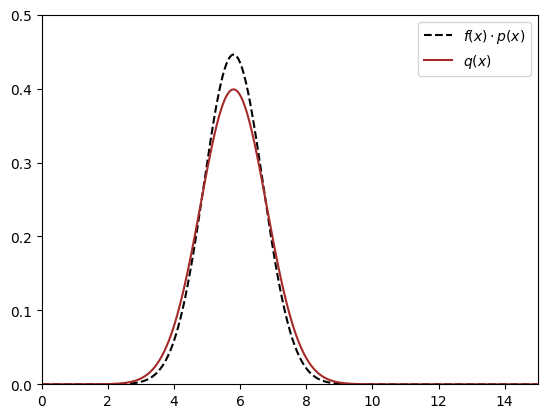
\includegraphics[width=0.4\linewidth]{addons/fp_and_q}
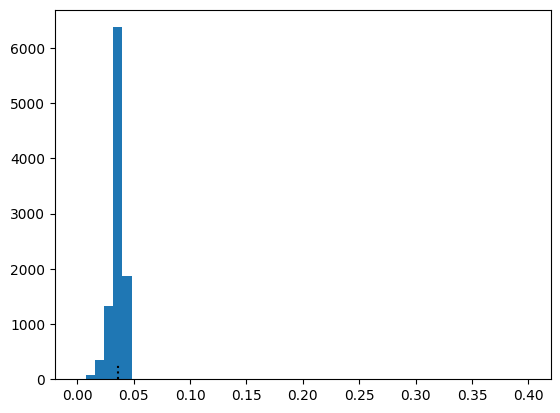
\includegraphics[width=0.4\linewidth]{addons/good_sampling}
\end{center}
\label{fig:fp_and_q}
\end{figure}

The resulting sampling is much better since the values are now clustered around 0.03. Comparing the estimates of the expectation in the two cases shows that the value is essentially the same, but the variance almost a factor 200 lower when using the importance sampling.
\begin{ioutput}
Numerical Simulation: mean 0.03611, variance 0.00759
Importance Sampling: mean 0.03603, variance 0.00003
\end{ioutput}
Note that in general it’s not trivial at all to find $q$, and certainly there are much more difficult real-word scenarios. For this example I actually plotted $p(x)f(x)$ and then picked a $q$ which resembled it best.

\begin{question}
Implement the importance sampling example outlined above, trying to reproduce the results quoted in the text.
\end{question}
\begin{question}
Estimate how unlucky is a 25 standard deviation return
\begin{equation*}
\theta := P(X\geq 25) = \mathbb{E}[\mathbbm{1}_{X\geq 25}]  \quad\text{where } X\sim \mathcal{N}(0, 1)
\end{equation*}
\end{question}
\begin{question}
Consider a one year ($T=1$) call option with $S_0=100$ , $K=170$,  $\sigma=0.2$, and $r=0.06$. The option is far out of the money, assuming we need to estimate its valye using Monte Carlo simulation, improve the efficiency of the calculation with importance sampling.

\noindent
Interesting reference \emph{Variance Reduction Techniques of Importance Sampling Monte Carlo Methods for Pricing Options}, 
Journal of Mathematical Finance, 2013, 3, 431-436.
\end{question}
\end{document}
